\section{Introduction}

A supervised machine learning problem is one which a learning algorithm is presented a set of training data and attempts to find an unknown function which maps the training values to the correct answer.
Typically the training set, denoted $S$, is a set of the form $\left \{ (\vec{x}_1,y_1), (\vec{x}_2,y_2), \dots, (\vec{x}_n,y_n) \right \}$ where $\vec{x}_i$ is vector of some features of the problem.
Problem features are generally discrete or real valued items.
Examples of problem features that could represent a person include height, weight, age, zip code, grade point average, starting salary, and telephone number.
The $y_i$ are the class of the training feature $\vec{x}_i$ belongs to; these might be University of Tennessee students or Carnegie Mellon students.
In this examples students with a zip code of 15213 are likely to be Tartans, while students with a zip code of 37916 are like to be Volunteers.
The challenge arises from examples have overlapping features; for example, this author as a former Tartan and current Vol would be difficult to classify by zip code.
The learning algorithm's job is then to find a hypothesis $h$ that correctly classifies a student as a Volunteer of Tartan based on the features provided.
This learning process can then be defined as finding the hypothesis that has the least error (incorrect classifications) on the training data set while extending to examples outside of the training space.

\subsection{Support Vector Machines}
Support Vector Machines (SVM) are a supervised learning technique in which hyperplanes are constructed in a high dimensional space to which the features are mapped.
SVMs find the hyperplanes that are the farthest away from all of mapped features in order to provide excellent training performance while still maintaining the ability to generalize to new instances; i.e. SVMs are maximal margin classifiers.
For a binary classification the decision function of the SVM is the dot product of the weight vector and the training example in the feature space added to a bias vector as shown in Equation \ref{eq:BCSVM}
\begin{equation}
\label{eq:BCSVM}
f \left ( \vec{x} \right ) = \left \langle \vec{w} , \phi(\vec{x}) \right \rangle + \vec{b}
\end{equation}
where $\phi(\vec{x})$ is a mapping to the higher dimensional space.
The SVM is then learning the optimal values of the weight vector $\vec{w}$ and the basis $\vec{b}$.

The radial basis function (Equation \ref{eq:RBF}) is a common kernel function used to map the input vector $\vec{x}$ into a higher dimension.
\begin{equation}
\label{eq:RBF}
k \left ( \vec{x}_i , \vec{x}_j \right ) = exp \left ( - \frac{\left \| \vec{x}_i - \vec{x}_j \right \|}{2\sigma^2} \right ) 
\end{equation}
The maximal margin is ensured by minimizing:
\begin{equation}
\label{eq:Min}
g(\vec{w},\eta) = \frac{1}{2} \left \| \vec{w} \right \| + C \sum_{i=1}^N \zeta_i
\end{equation}
subject to:
\begin{equation}
\label{eq:Constraint}
y_i( \left \langle \vec{w},\phi(\vec{x}) \right \rangle + b ) \ge 1-\zeta_i, ~~~\zeta_i \ge 0
\end{equation}
where $\zeta_i$ is the $i$th slack variable and C is the regularization parameter \cite{li_adaboost_2008}.
This problem can be translated  in to the Wolfe dual form, which can be solved with quadratic programing \cite{li_adaboost_2008}.

\subsection{Boosting}
Unbalanced data sets (data sets in which a majority of the values come from one class, see Figure \ref{fig:ClassDist}) are difficult for classification schemes to learn because the minority class is not well represented and tends to be thought as noise for the classifier.
Often classifiers are trained from unbalanced data sets by artificially balancing the data set by sampling techniques; i.e. up-sampling (sampling more from the minority class) and down-sampling (sampling less from the majority class).
Boosting is an ensemble learning method in which a set of weights is maintained over the training samples and adaptively adjusted after each training iteration according to the ones that are misclassified \cite{li_adaboost_2008}.
Given an individual classifier $h$, an ensemble of classifiers can be constructed of a set of individual classifiers, $H=\{h_1, h_2,\dot, h_n\}$.
By maintaining a weight distribution over all of the training examples, these weights could be updated to emphasize the training examples that are misclassified incorrectly.  These incorrectly classified examples could then be learned in a refinement of the classifier or by training adding a new classifier to the ensemble with the new weights.
Performance of the ensemble is enhanced as long as the individual classifiers are weak and have uncorrelated errors, as when any single classifier is incorrect the other classifiers in the ensemble might correctly classify the example.
\begin{figure*}[ht!]
	\centering
	\begin{subfigure}[b]{0.3\textwidth}
		\centering
		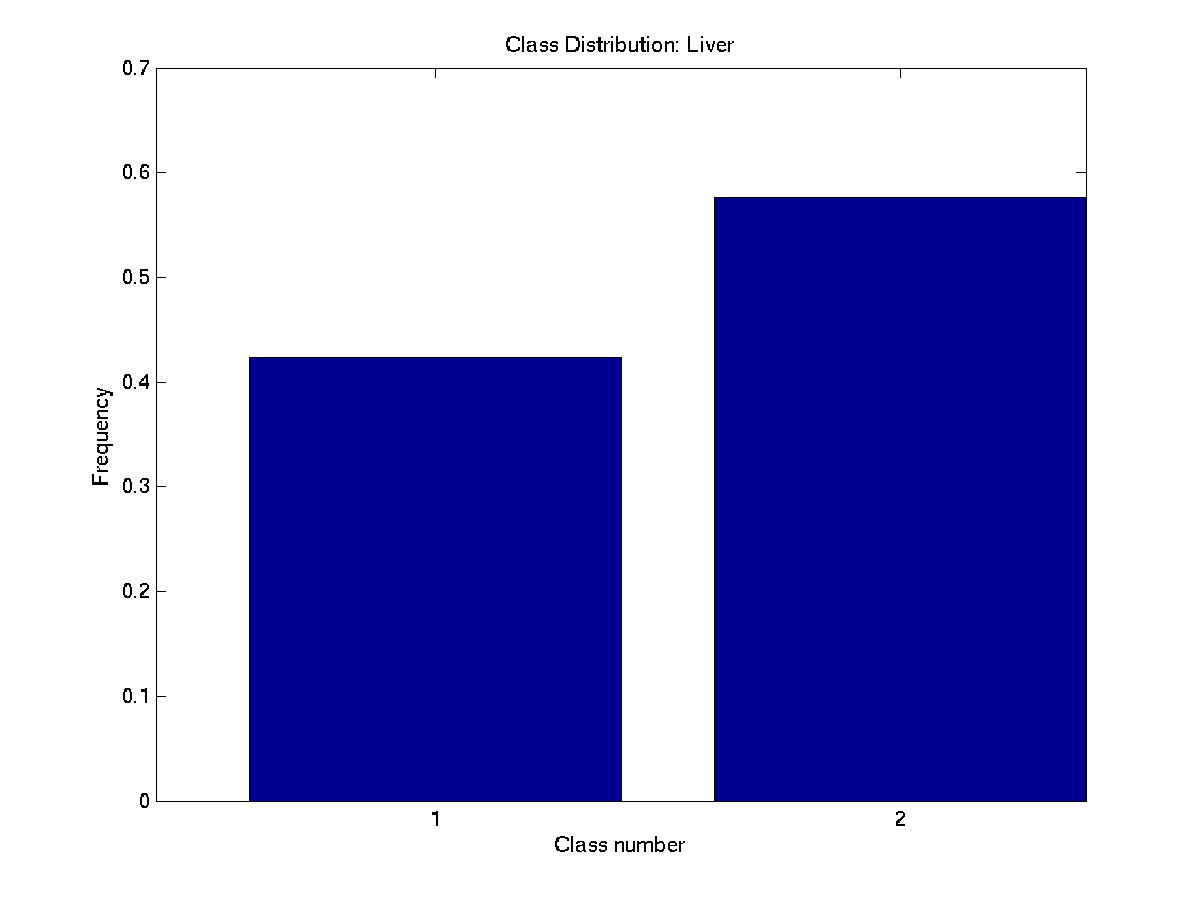
\includegraphics[width=\textwidth]{Liver_ClassDist}
        \caption{Liver}
	\end{subfigure}%
	~
	\begin{subfigure}[b]{0.3\textwidth}
		\centering
		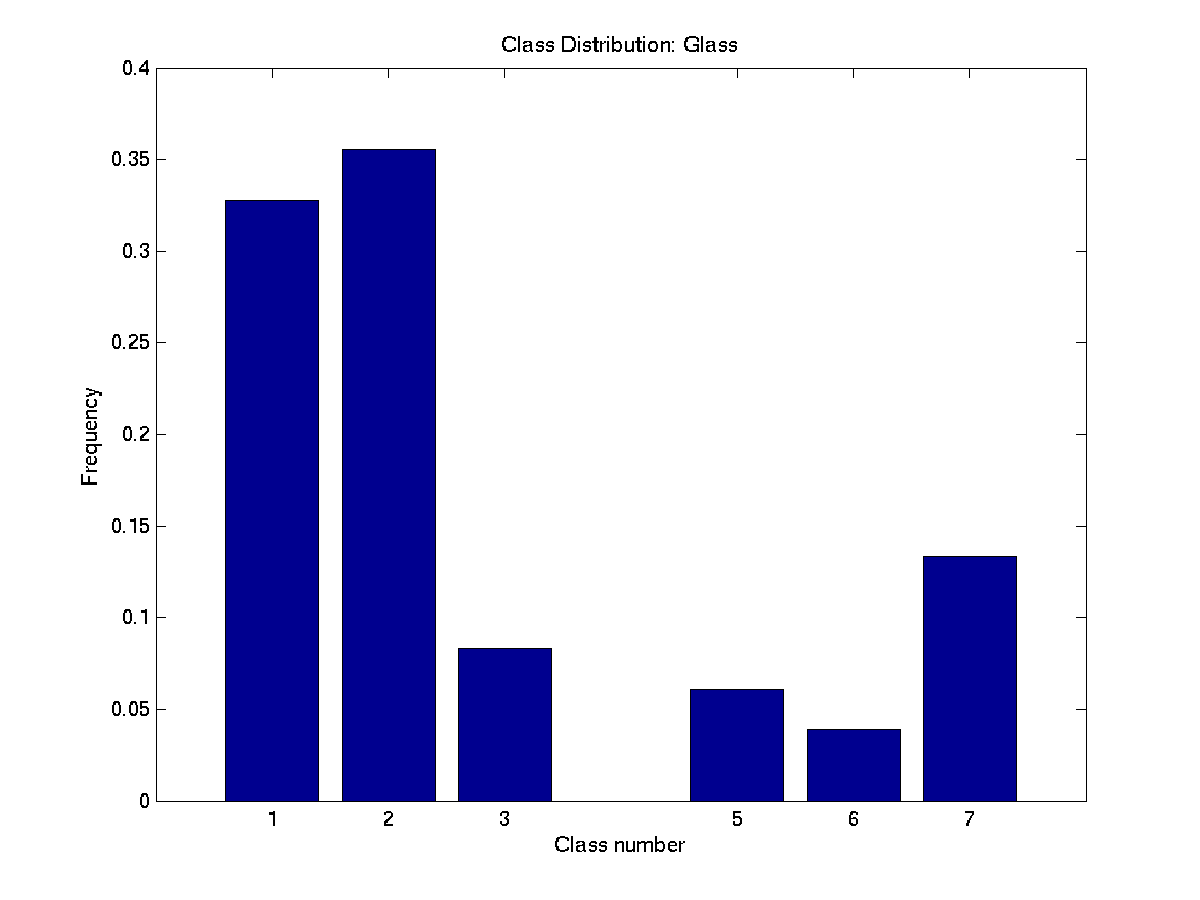
\includegraphics[width=\textwidth]{Glass_ClassDist}
        \caption{Glass}
	\end{subfigure}	
    ~
	\begin{subfigure}[b]{0.3\textwidth}
		\centering
		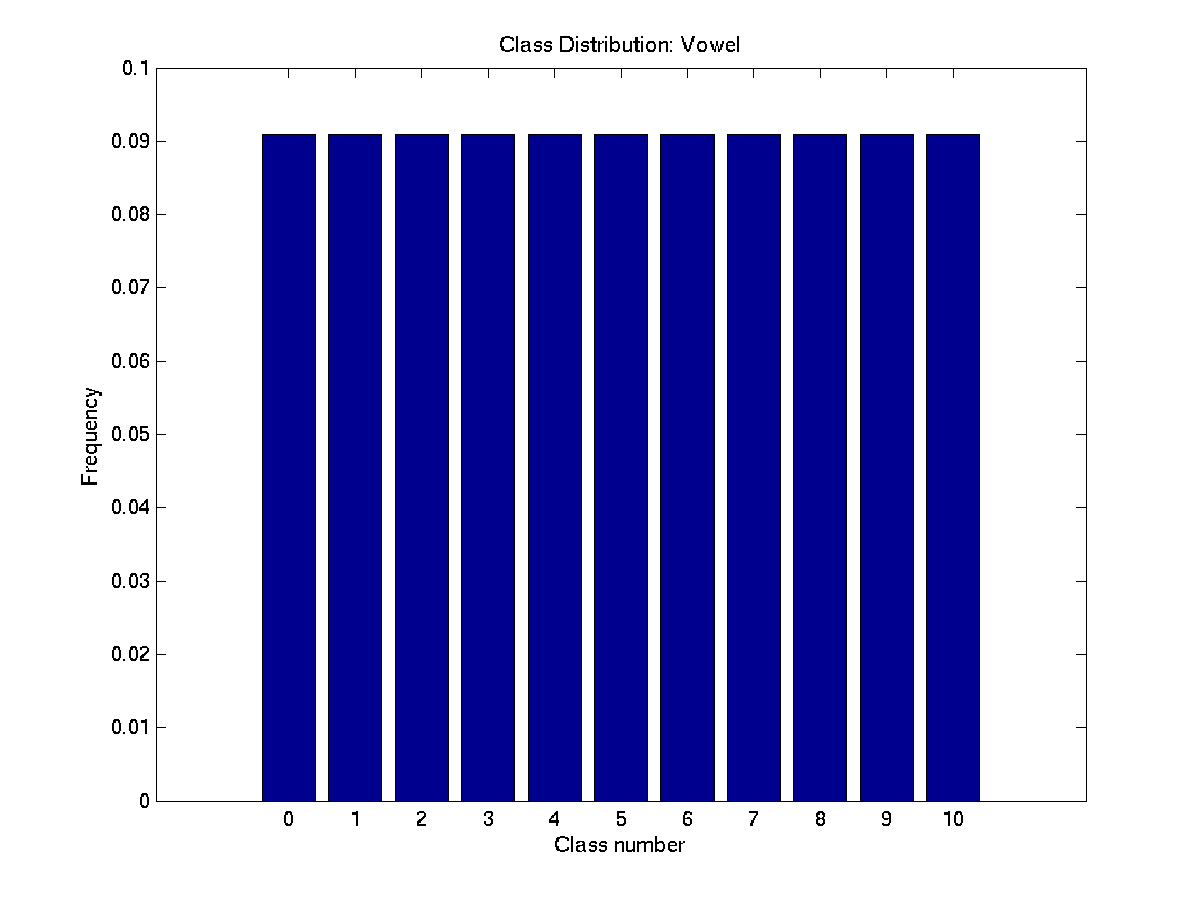
\includegraphics[width=\textwidth]{Vowel_ClassDist}
        \caption{Vowel}
	\end{subfigure}%
	\caption{Distribution of Class Data}
	\label{fig:ClassDist}
\end{figure*}
